\chapter{Ethik}
\label{chap:ethics}

In diesem Kapitel werde ich die Ethik im zusammenhang zur KI beschreiben.

\section{Was ist Ethik?}

thik ist jener Teilbereich der Philosophie, der sich mit den Voraussetzungen und der Bewertung menschlichen Handelns befasst. \textit{" Die (allgemeine) Ethik wird heute als die philosophische Disziplin verstanden, die Kriterien für gutes und schlechtes Handeln und für die Bewertung seiner Motive und Folgen aufstellt. Sie ist von ihrer Zielsetzung her eine praktische Wissenschaft." \citep{ethics-wikipedia}}

\section{Warum die KI schlecht und gut nicht unterscheiden kann}

Man unterscheidet zwischen richtig und falsch, indem man sich an bestimmte Werte und Gesetze hält. Zum Beispiel wird das Überqueren einer roten Ampel als falsch angesehen, da es gegen das Gesetz verstößt. Es geht also darum, sich an moralische und gesetzliche Normen zu halten, um zwischen richtigem und falschem Handeln zu unterscheiden. Für die KI ist egal ob etwas schlecht oder gut ist, weil es ihr so beigebracht wurde zu handeln, wenn man einer KI beibringt, dass töten gut sei. Diese KI würden dann glauben, dass diese Aussage stimmt und würde sie unter gar keinen Umständen hinterfragen, wie es Menschen machen würden.

\begin{figure}[h]
    \centering
    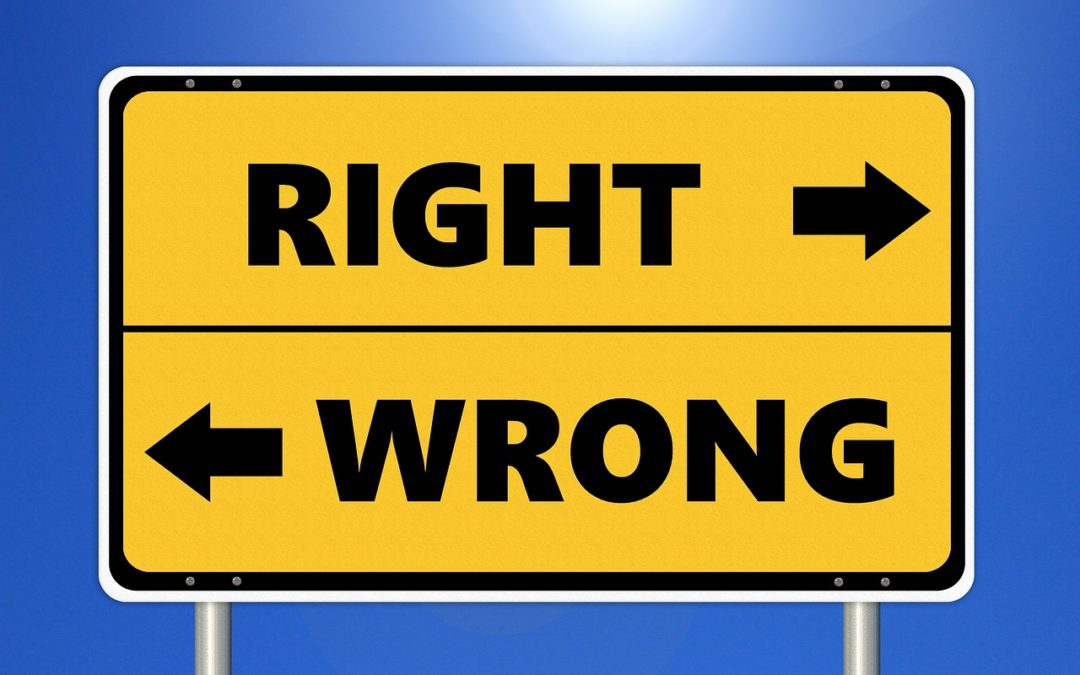
\includegraphics[width=0.5\textwidth]{ethics.jpg}
    \caption{Ein Schild beschrieben mit richtig und falsch}
    \label{fig:ethics}
\end{figure}

\section{Das Trolley Problem}

Ein gutes Beispiel, bei welchem die KI probleme hätte. Das Trolley-problem ein sehr bekanntes Dilemma. Es handelt sich um sechs Personen, auf der einen Schiene sind fünf Personen, auf der abzweigung ist eine Person. Wenn jetzt eine KI, welche trainiert ist Menschen zu beschützen, in so einem Geschehen vorkommen würde. Das Trolley-Problem ist bekannt, weil den Hebel betätigen würde heissen, man hat dafür gesorgt das eine Person umgebracht wurde, jedoch ist man dann Schuld für diesen Tot. Ignoriert man das Geschehen werden fünf Personen umgebracht, man ist zwar nicht Schuld aber man hätte dies verhindern können. Eine KI hätte hier grosse Mühe oder würde denn logischten weg berechnen, der jedoch unmoralisch ist. \textit{"bei denen intuitiv die Rettung von fünf Menschen auf Kosten von einem Menschenleben unzulässig erscheint. Diese Erklärungslücke bezeichnet Judith Jarvis Thomson als Trolley-Problem und stellt dem Weichenstellerfall dazu" \citep{trolley-problem-wikipedia}}

\begin{figure}[h]
    \centering
    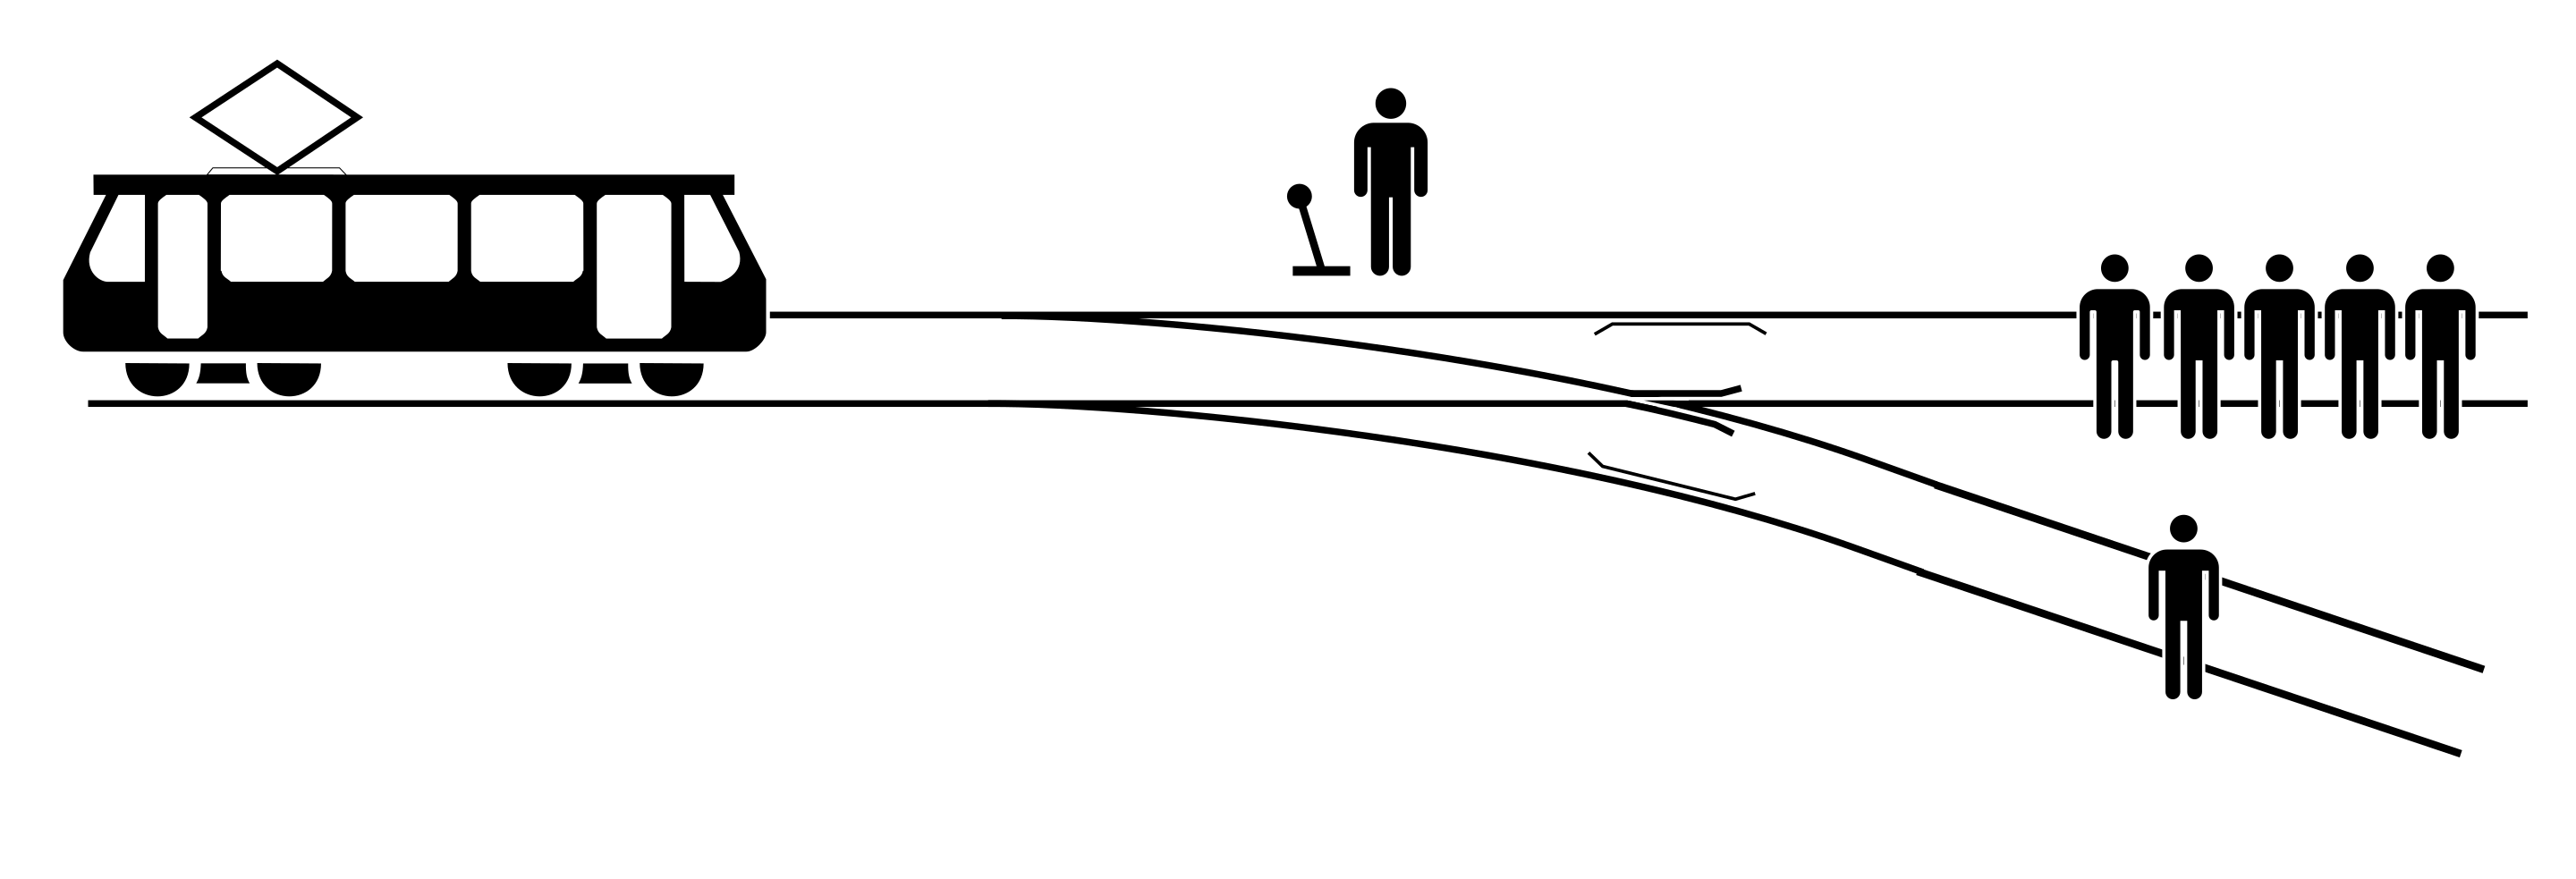
\includegraphics[width=0.5\textwidth]{Trolley_Problem.png}
    \caption{Das Trolley Problem}
    \label{fig:trolley_problem}
\end{figure}